\subsection{Background}
\textbf{Sequence-to-sequence language models} such as BART \cite{lewis-etal-2021-paq}, T5 \cite{Raffel2020ExploringTL}, and PEGASUS \cite{Zhang2020PEGASUSPW} combine transformer encoders and decoders to produce models which can adapt to novel tasks and reach top performance on tasks ranging from information retrieval \cite{Nogueira2020DocumentRW} to summarization \cite{Raffel2020ExploringTL}. \\
We focus on the instruction-tuned FLAN-T5 models \cite{Wei2021FinetunedLM} as their performance is competitive and they feature wide variations in model size ranging from 60 million to 11 billion parameters and given the cost of training the larger variants, focus on the small, base, and large variants. Details on model size and architecture can be found in table \ref{tab:models}.\\
\textbf{Abstractive summarization} is a method of sequence compression where a source document $D$ is transformed into a target document $d_{sum}$, which is shorter but faithful to the input. \\
Using a sequence-to-sequence model such as T5 \cite{Raffel2020ExploringTL}, a transformer-based encoder (enc) produces a contextual document representation $e$, and a transformer-based decoder generates $d_{sum}$ one token at a time conditioned on $e$. Models are initially pre-trained in a self-supervised fashion and then fine-tuned using a set of source and target documents where each document $d \in D$ contains a $d_{sum}$, which is both shorter than $d$ and true to the source. \\
\textbf{Datasets} of use are a combination of public and academic benchmarks and a proprietary web search dataset. The CNN/DailyMail (CNNDM) \cite{see-etal-2017-get} and XSUM \cite{Narayan2018DontGM} datasets are based on the summarization of English new language models. The Query Independent Web Summary (QIWS) is a proprietary corpus of abstractive summaries of web pages that are used to create informative contextual snippets for search engine users. It is important to note the differences in compression factor in each dataset as each impact how decoder-driven inference latency is. Further information on the makeup of each dataset can be found in table \ref{tab:datasets} \\
\begin{table*}[!ht]
    \centering
    \small
    \caption{Impact of scale on inference throughput for abstractive summarization models trained on the XSUM dataset. Latency is measured in MS/batch and the impact is the impact to latency vs. the small model}
    \begin{tabular}{|l|l|l|l|l|l|l|l|l|}
    \hline
         Model & R-2 & Gain & BS 1 Latency & Impact & BS 8 Latency & Impact & BS 16 Latency & Impact \\ \hline
        small & 17.55 & 0.00\% & 138 & 1 & 230 & 1 & 330 & 1 \\ \hline
        base & 19.77 & 12.63\% & 199 & 1.44 & 550 & 2.39 & 931 & 2.82 \\ \hline
        large & 21.15 & 20.51\% & 445 & 3.22 & 1480 & 6.43 & 2700 & 8.18 \\ \hline
    \end{tabular}
    \label{tab:cnndm-scale-inference}
\end{table*}
\begin{table*}[!ht]
    \centering
    \small
    \caption{Impact of scale on inference throughput for abstractive summarization models trained on the QIWS dataset. Latency is measured in MS/batch and the impact is the impact to latency vs. the small model}
    \begin{tabular}{|l|l|l|l|l|l|l|l|l|}
    \hline
        Model & R-2 & Gain & BS 1 Latency & Impact & BS 8 Latency & Impact & BS 16 Latency & Impact \\ \hline
        small & 29.03 & 0 & 524 & 1 & 653 & 1 & 729 & 1 \\ \hline
        base & 34.19 & 17.77\% & 746 & 1.42 & 1060 & 1.62 & 1310 & 1.80 \\ \hline
        large & 37.37 & 28.72\% & 1,430 & 2.73 & 2240 & 3.43 & 3320 & 4.55 \\ \hline
    \end{tabular}
    \label{tab:qiws-scale-inference}
\end{table*}
\begin{table*}[!ht]
    \centering
    \small
    \caption{Impact of scale on inference throughput for abstractive summarization models trained on the CNNDM dataset.Latency is measured in MS/batch and the impact is the impact to latency vs. the small model}
    \begin{tabular}{|l|l|l|l|l|l|l|l|l|}
    \hline
         Model & R-2 & Gain & BS 1 Latency & Impact & BS 8 Latency & Impact & BS 16 Latency & Impact \\ \hline
        small & 11.09 & 0 & 171 & 1.00 & 252 & 1.00 & 344 & 1.00 \\ \hline
        base & 15.69 & 41.50\% & 255 & 1.49 & 550 & 2.18 & 845 & 2.46 \\ \hline
        large & 16.34 & 47.41\% & 525 & 3.07 & 1370 & 5.44 & 2300 & 6.69 \\ \hline
    \end{tabular}
    \label{tab:xsum-scale-inference}
\end{table*}
\begin{figure}
    \centering
    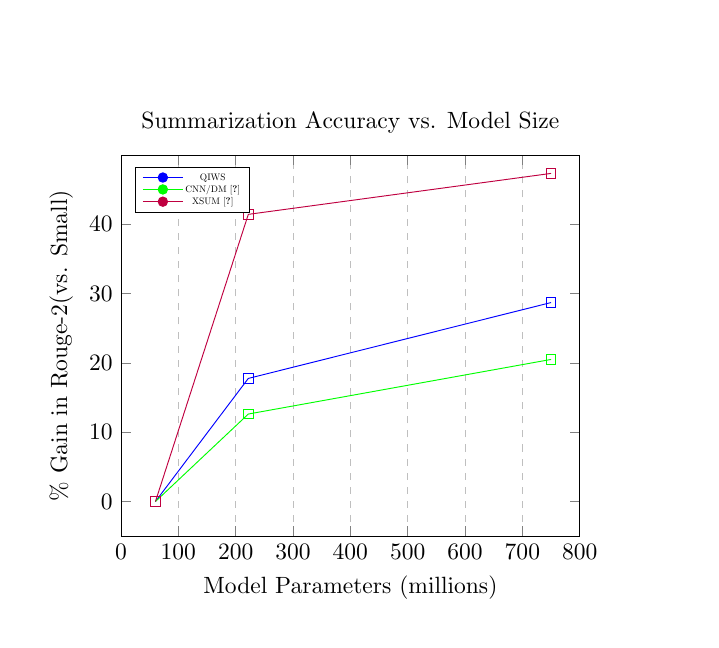
\begin{tikzpicture}
\scalebox{0.85}{
\begin{axis}[
    title={Summarization Accuracy vs. Model Size},
    ylabel={\% Gain in Rouge-2(vs. Small)},
    xlabel={Model Parameters (millions)},
    ymin=-5, ymax=50,
    xmin=0, xmax=800,
    ytick={0,10,20,30,40},
    xtick={0,100,200,300,400,500,600,700,800},
    legend pos=north west,
    xmajorgrids=true,
    grid style=dashed,
    legend style={nodes={scale=0.4, transform shape}}, 
    legend image post style={mark=*}
]
\addplot[
    color=blue,
    mark=square,
    ]
    coordinates {
    (60,0) ( 222,17.77) (750,28.72) 
    };
\addplot[
    color=green,
    mark=square,
    ]
    coordinates {
    (60, 0) (222, 12.63) (750,20.51)
    };  
\addplot[
    color=purple,
    mark=square,
    ]
    coordinates {
    (60,0) (222, 41.45) (750,47.36)
    };
\legend{QIWS, CNN/DM \cite{see-etal-2017-get}, XSUM \cite{Narayan2018DontGM} }
 \end{axis}}
\end{tikzpicture}
    \caption{Model Size vs. Gain to summarization accuracy as measured by the relative Gain in rouge-2 vs. the small model.}
    \label{fig:scale-laws}
\end{figure}
\textbf{Metrics} For each dataset, we evaluate model performance by measuring the ROUGE-1 (R-1), ROUGE-2 (R-2), ROUGE-L (R-L), RougeSum-L (RSL) \footnote{Rouge-L is sentence level vs. RougeSum-L is summary level} \cite{lin-2004-rouge}, and Generation Length (GenL) on the test portion of the dataset. To aid the reproducibility and extension of our work, we experiment using HuggingFace's Transformers \footnote{https://github.com/huggingface/transformers}, release our training and pruning scripts \footnote{https://github.com/spacemanidol/Efficient-Web-Scale-Absractive-Summarization} and model variants for datasets that are publicly available datasets  \footnote{https://huggingface.co/spacemanidol}. 
\subsection{Scaling Laws for Abstract Summarization}
To study the role of scale in abstractive summarization, we train small, base, and large models of the three datasets mentioned above. We do not study the XL (3B) and XXL (11B) as they are expensive and slow to train.\\ For all of our experiments, we train on various hardware but fix the batch size to 64 using gradient accumulation and leverage the hyperparameters in \ref{tab:hyperparams-transfer}. While further hyperparameter optimization and instruction tuning would likely lead to further gains in accuracy, our work is not focused on absolute Gains but on the relative relation of scale.  \\

As shown in \ref{fig:scale-laws}, \ref{tab:scale-qiws}, \ref{tab:scale-cnndm}, and \ref{tab:scale-xsum}, there is a substantial role between scale and performance, but there is a substantial variation across datasets. \\
Datasets with short candidate summaries, such as XSUM, see nearly three times the impact compared to the long summaries of QIWS and XSUM. During qualitative evaluations, the role of scale can easily be observed as smaller models generate more short keyword summaries while introducing scale makes responses more natural. 
\begin{table}[!ht]
    \centering
    \tiny
    \caption{Relation between scale and asymmetry on model performance on the QIWS dataset}
    \scalebox{0.9}{
    \begin{tabular}{|l|l|l|l|l|l|l|l|}
    \hline
        \multicolumn{2}{l}{} &  \multicolumn{2}{l}{Small} & \multicolumn{2}{l}{Base} & \multicolumn{2}{l}{Large}  \\ \hline 
        $l_{enc}$ & $l_{dec}$ & R-2 & $R$ & R-2 & $R$ & R-2 & $R$ \\ \hline
        6 & 6 & 29.03 & 100.00\% & 34.19 & 100.00\% & 37.37 & 100.00\% \\ \hline
        6 & 5 & 28.90 & 99.55\% & 34.00 & 99.44\% & 37.59 & 100.59\% \\ \hline
        6 & 4 & 28.56 & 98.40\% & 34.50 & 100.91\% & 36.56 & 97.84\% \\ \hline
        6 & 3 & 27.94 & 96.24\% & 33.70 & 98.58\% & 35.74 & 95.64\% \\ \hline
        6 & 2 & 24.85 & 85.61\% & 31.93 & 93.38\% & 35.13 & 94.01\% \\ \hline
        6 & 1 & 15.41 & 53.08\% & 28.05 & 82.03\% & 33.69 & 90.15\% \\ \hline
        \midrule
        5 & 6 & 27.92 & 96.17\% & 33.57 & 98.18\% & 36.39 & 97.38\% \\ \hline
        4 & 6 & 27.75 & 95.60\% & 33.06 & 96.69\% & 35.90 & 96.07\% \\ \hline
        3 & 6 & 25.20 & 86.82\% & 32.23 & 94.28\% & 34.22 & 91.58\% \\ \hline
        2 & 6 & 23.67 & 81.55\% & 27.47 & 80.35\% & 33.42 & 89.43\% \\ \hline
        1 & 6 & 18.23 & 62.79\% & 25.57 & 74.78\% & 30.31 & 81.11\% \\ \hline
        \midrule
        5 & 5 & 26.82 & 92.38\% & 32.88 & 96.18\% & 36.32 & 97.20\% \\ \hline
        4 & 4 & 26.62 & 91.72\% & 32.81 & 95.96\% & 35.98 & 96.29\% \\ \hline
        3 & 3 & 23.12 & 79.64\% & 28.70 & 83.95\% & 33.00 & 88.31\% \\ \hline
        2 & 2 & 19.14 & 65.92\% & 26.53 & 77.60\% & 30.78 & 82.38\% \\ \hline
        1 & 1 & 6.09 & 20.99\% & 19.64 & 57.43\% & 22.77 & 60.94\% \\ \hline
    \end{tabular}}
    \label{tab:qiws-r2-asym}
\end{table}
\subsection{Inference Benchmark}
To evaluate the impact of asymmetry on inference, we run experiments on the throughput of each model. Using an A10 GPU and the models from our QIWS datasets, we evaluate performance with a max sequence length of 1024, a max summary of 256, and batch sizes 1, 8, and 16 using native inference in PyTorch. We report the mean and standard deviation of timings on seven runs. \\
In comparing the impact of scale on R-2 vs. the effects on latency across batch sizes in \ref{tab:cnndm-scale-inference}, \ref{tab:xsum-scale-inference}, \ref{tab:qiws-scale-inference} it becomes clear that larger models are more expensive to execute significantly as batch sizes increase. This is because of potential differences in output length within a batch as the batch completes when all sequences have produced an \textit{EOS} token. To alleviate this issue bottleneck, improved streaming methods for improved batching have been proposed \cite{Yang2020ASA} but can be challenging to manage. 